\chapter[Avaliação do Questionário]{Avaliação do Questionário}

Os tipos de questionários abordados referem-se aos tipos de perguntas feitas para os usuários após a utilização do sistema.  Foi elaborado um questionário com base em perguntas que auxiliem ao usuário a expressar sua opinião sobre a utilização do sistema.
As questões do tipo fechadas expõem a análise dos resultados através de escalas, pois são facilmente mapeadas para números, embora restrinjam as possibilidades de resposta dos usuários. 

Para a análise, fizemos a relação das perguntas dos questionários com as metas de usabilidade, a fim de verificarmos se foi atingido o objetivo para determinada meta de acordo com a relação dos resultados do questionário.

\begin{table}[H]
	\centering
	\begin{tabular}{|c|c|}
		\hline 
		\textbf{Metas} & \textbf{Itens do Questionário}\tabularnewline
		\hline 
		\hline 
		\textbf{Flexibilidade e eficiência no uso:} & 1, 2, 3, 5, 6, 10, 14, 17, 18\tabularnewline
		\hline 
		\textbf{Reconhecer ao invés de lembrar:} & 7, 8, 9, 11, 12, 13, 15, 16\tabularnewline
		\hline 
		\textbf{Agradável:} & 4, 21, 23\tabularnewline
		\hline 
		\textbf{Proveitoso:} & 19 ,20 ,22\tabularnewline
		\hline 
	\end{tabular}
	\caption{Metas de Usabilidade x Perguntas Questionário}
	\label{Metas_x_Questionario}
\end{table}

\subsection{Questionário}

O questionário foi aplicado de forma a se obter um retorno das respostas dos usuários em escala, sempre mantendo um padrão para não deixar o entrevistado confuso, as respostas são dispostas de maneira semelhante a escala \textit{Lickert} com pontuação de 0 a 5, indo de Concordo Totalmente (5 pontos) até Discordo Totalmente (1 ponto) e Não se aplica (0 ponto). As perguntas são feitas de maneira objetivas e claras, sempre no formato que possibilite ao usuário respondê-las de acordo com as opções disponíveis.

\hspace{1.3cm}
\textbf{Perguntas:}

\begin{enumerate}
	\item A interface do sistema de busca avançada do site é boa?
	\item O tempo de resposta do site é rápido?
	\item Foi fácil sair ou voltar dentro do site?
	\item Você se sente a vontade ao utilizar o site?
	\item Você consegue visualizar bem o conteúdo do site?
	\item O site permite você alternar facilmente entre as menus ou telas?
	\item Os textos presentes no site auxiliam na navegação do mesmo?
	\item As imagens presentes no site auxiliam na navegação do mesmo?
	\item Ficou clara a proposta do site?
	\item Este sistema contém o conteúdo suficiente para o propósito dele? 
	\item Qualquer pessoa navegar no site com facilidade?
	\item A organização do conteúdo do site é boa?
	\item É fácil saber em que página você está dentro do site?
	\item O site não impõe qualquer interrupção desnecessária em sua sua navegação
	\item Foi fácil aprender a utilizar o site?
	\item Depois de utilizar o site, você não precisaria se esforçar pra lembrar como utilizá-lo novamente?
	\item Quando você clica em um link ou botão, o site direciona você para onde deveria realmente ir?
	\item Você encontra informações importantes no topo da página?
	\item É agradável usar este material com outro colega no mesmo computador?
	\item Você, ao utilizar este material, acabou se aprofundando tanto que sentiu que o tempo passou muito rápido?
	\item É prática a navegação do site?
	\item Não é difícil entender o que se deve fazer no site?
	\item Você recomendaria esse site para outra pessoa?
\end{enumerate}


\subsection{Resultado}

Baseado nas heurísticas que se desejamos alcançar, foi criado um formulário, usando o Google Forms, apenas com as questões que remetem a elas. Dessa forma, foi possível  rastrear a evolução da usabilidade entre as versões dos protótipos. Foram separadas as perguntas em dois grupos, aquelas que evidenciam uma avaliações negativas de nosso sistema e aquelas que evidenciam uma boa experiência de usabilidade em nosso sistema. O usuário então enumera de 1 a 5 o quanto aquela frase corresponde a realidade na sua experiênca que teve ao testar o protótipo.

Foram adquiridos os feedbacks dos usuários durante as etapas da prototipação, solicitando que estes, após utilização do protótipo fizessem um questionário, sobre a experiência que obtiveram durante a utilização do possível sistema.

\begin{table}[H]
	\centering
	\begin{tabular}{|c|c|}
		\hline 
		\textbf{Alternativas} & \textbf{Quantidade}\tabularnewline
		\hline 
		\hline 
		Concordo plenamente & 22\tabularnewline
		\hline 
		Concordo & 75\tabularnewline
		\hline 
		Neutro & 36\tabularnewline
		\hline 
		Discordo & 17\tabularnewline
		\hline 
		Discordo Plenamente & 0\tabularnewline
		\hline 
		Não se aplica & 11\tabularnewline
		\hline 
	\end{tabular}
	\caption{Baixa fidelidade - 7 Entrevistados}
	\label{Metas_x_Questionario}
\end{table}

\begin{figure}[H]
	\begin{center}
		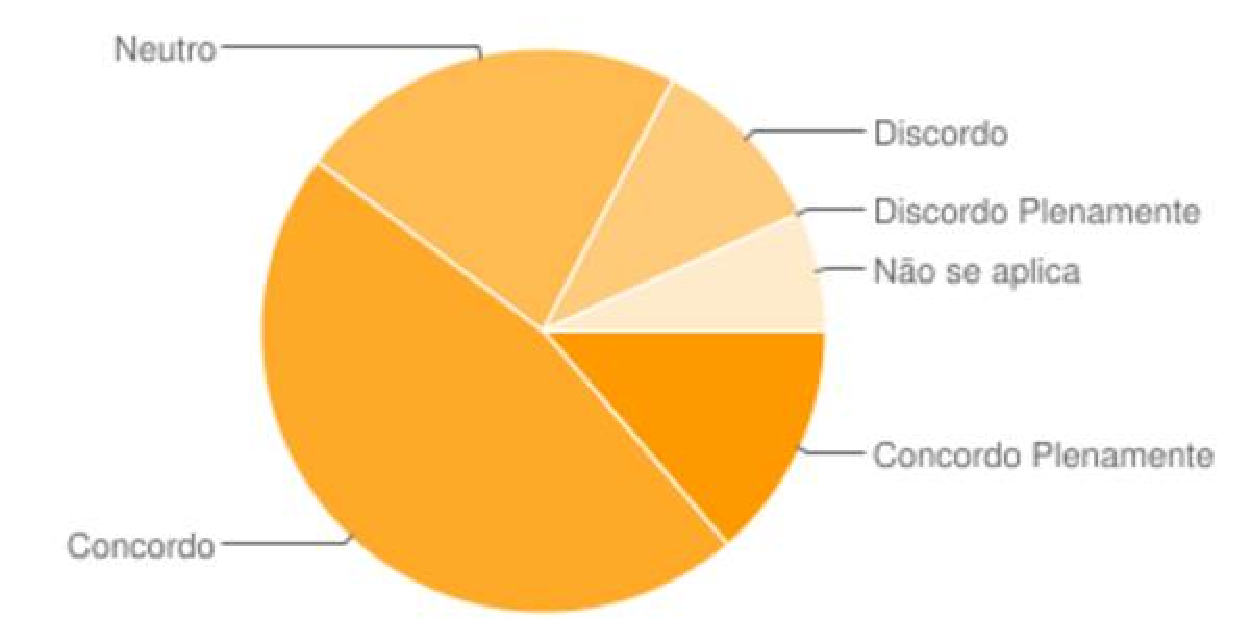
\includegraphics[keepaspectratio,scale=0.6]{figuras/grafico_questionario_baixa_fidelidade.eps}
		\caption{Gráfico: Questionário Baixa Fidelidade}
	\end{center}
\end{figure}

\begin{table}[H]
	\centering
	\begin{tabular}{|c|c|}
		\hline 
		\textbf{Alternativas} & \textbf{Quantidade}\tabularnewline
		\hline 
		\hline 
		Concordo plenamente & 64\tabularnewline
		\hline 
		Concordo & 15\tabularnewline
		\hline 
		Neutro & 8\tabularnewline
		\hline 
		Discordo & 5\tabularnewline
		\hline 
		Discordo Plenamente & 1\tabularnewline
		\hline 
		Não se aplica & 7\tabularnewline
		\hline 
	\end{tabular}
	\caption{Média fidelidade - 4 Entrevistados}
	\label{Metas_x_Questionario}
\end{table}

\begin{figure}[H]
	\begin{center}
		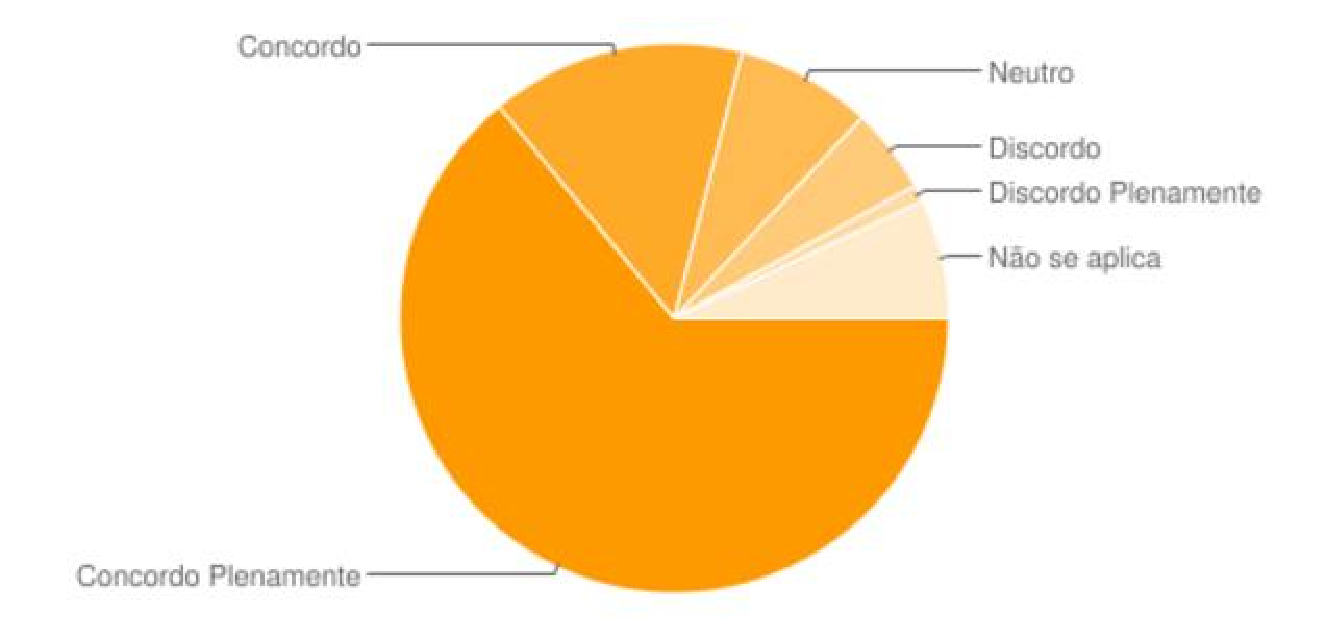
\includegraphics[keepaspectratio,scale=0.6]{figuras/grafico_questionario_media_fidelidade.eps}
		\caption{Gráfico: Questionário Média Fidelidade}
	\end{center}
\end{figure}

\begin{table}[H]
	\centering
	\begin{tabular}{|c|c|}
		\hline 
		\textbf{Alternativas} & \textbf{Quantidade}\tabularnewline
		\hline 
		\hline 
		Concordo plenamente & 43\tabularnewline
		\hline 
		Concordo & 18\tabularnewline
		\hline 
		Neutro & 4\tabularnewline
		\hline 
		Discordo & 0\tabularnewline
		\hline 
		Discordo Plenamente & 0\tabularnewline
		\hline 
		Não se aplica & 4\tabularnewline
		\hline 
	\end{tabular}
	\caption{Alta fidelidade - 3 Entrevistados}
	\label{Metas_x_Questionario}
\end{table}

\begin{figure}[H]
	\begin{center}
		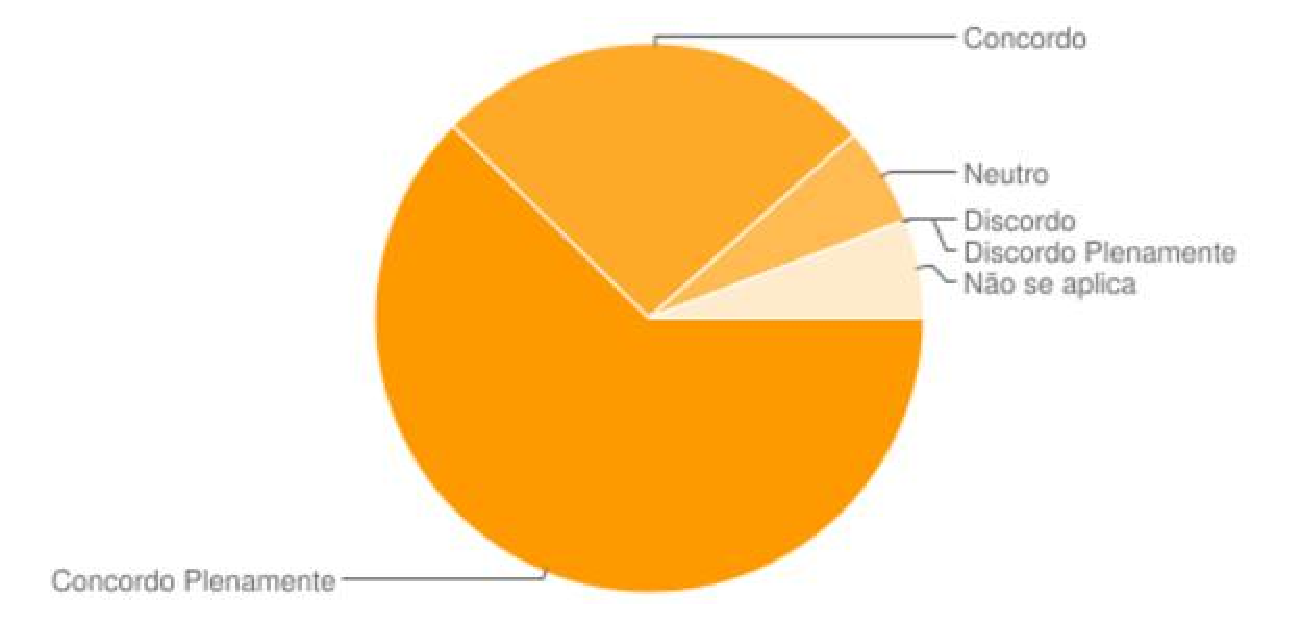
\includegraphics[keepaspectratio,scale=0.6]{figuras/grafico_questionario_alta_fidelidade.eps}
		\caption{Gráfico: Questionário Alta Fidelidade}
	\end{center}
\end{figure}